\documentclass[10pt,a4paper,openright,twoside]{C:/Didattica/git/lab2014Bo/it.unibo.iss2015intro/docsInternal/contents/llncs}
\setcounter{tocdepth}{3}
\setcounter{secnumdepth}{3}

%%%%%%%%%%%%%%%%%%%%%%%%%%%%%%%%%%%%%%%%%%%%%%%%%%%%%%%%%%%
%% package sillabazione italiana e uso lettere accentate
%%\usepackage[latin1]{inputenc}
\usepackage[english]{babel}
\usepackage[T1]{fontenc}
\usepackage{listings}
\usepackage{hyperref}
%%\usepackage{pdfpages}
%%\usepackage{amsmath,amsfonts,amssymb,amsthm}
\usepackage{fancyhdr}   %%% by AN for page number position
%%%%%%%%%%%%%%%%%%%%%%%%%%%%%%%%%%%%%%%%%%%%%%%%%%%%%%%%%%%%%
  
\usepackage{url}
\usepackage{xspace}

\pagestyle{fancy}
\fancyhf{}
\rfoot{\thepage}

\makeatletter
%%%%%%%%%%%%%%%%%%%%%%%%%%%%%% User specified LaTeX commands.
\usepackage{../manifest}
\usepackage{amssymb}    %%% by AN
\usepackage{fancyvrb}   %%% by AN
\usepackage{floatflt}   %%% by AN\\
\usepackage{hyperref} 
%%\usepackage{graphicx}
\usepackage{color}
%% \usepackage[usenames,dvipsnames,svgnames,table]{xcolor}
\makeatother

\definecolor{goldenrod}{RGB}{255, 255, 204}
\definecolor{goldenrod2}{RGB}{255, 255, 153}
\definecolor{eclipseKeyword}{RGB}{149, 0, 85}
\definecolor{eclipseComment}{RGB}{83,128,64}
\definecolor{eclipseString}{RGB}{42, 0, 255}
\definecolor{lightgray}{rgb}{0.98,0.98,0.98}
\definecolor{mygreen}{RGB}{83,128,64}
\definecolor{mygray}{rgb}{0.5,0.5,0.5}
\definecolor{mymauve}{rgb}{0.58,0,0.82}

\newcommand{\code}[1]{{\color{blue}{\texttt{#1}}}}
\newcommand{\bt}[1]{{\color{magenta}\texttt{#1}}}
\newcommand{\fname}[1]{{\color{magenta}\texttt{#1}}}
\newcommand{\isa}{{\color{black}\texttt{ISA-95}}}
\newcommand{\opc}{{\color{black}\texttt{OPC-UA}}}


\lstnewenvironment{javacode}{\lstset{language=Java}}{}
\lstnewenvironment{qacode}{\lstset{language=qa}}{}

\lstdefinelanguage{Lisp}
{ morekeywords={require, var, function, for, while, if, new, return, else}
}
 
\lstdefinelanguage{contact}
{
 morekeywords={ContactSystem,Subject,Dispatch,forward,to,serve,BehaviorOf,
 var,action,state,initial,set,exec,call,doOut,endstate,goToState,onMessage,transitTo,doIn,external,context,
  Context, Signal, Event, emit, sense, if, Request, demand, grant}
}
\lstdefinelanguage{xtend}
{
 morekeywords={package, import, public, protected, private, class, override, void, def, dispatch, for, typeof}
}
\lstdefinelanguage{iot}
{
 morekeywords={Behavior, RobotSystem, ip, state, initial, endstate,goToState, package, import, public, protected, private, class, override, void, def, dispatch, for, typeof}
}

\lstset {
  language=contact,
  basicstyle={\scriptsize\ttfamily},
  %%numbers=left,
  backgroundcolor=\color{lightgray},
  showstringspaces=false,
  columns=flexible,
  keywordstyle={\color{eclipseKeyword}\textbf},
  commentstyle={\color{eclipseComment}\textit},
  stringstyle={\color{eclipseString}},
  frame=single,
  breaklines=true,
  breakatwhitespace=true,
  tabsize=4,
  morekeywords={ContactSystem,RobotSystem,Subject,Dispatch,forward,to,serve,Behavior,BehaviorOf,var,action,state,initial,set,exec,call,doOut,endstate,goToState,onMessage,transitTo,doIn,external,context,
  Context, Signal, Event, emit, sense, if}, 
  ndkeywords={Task,BehaviorOf,Event},
  ndkeywordstyle={\color{darkgray}\bfseries},
  escapeinside={(*@}{@*)},
  captionpos=b
}

\lstset{
  language=Lisp,
  basicstyle={\scriptsize\ttfamily},
  numbers=left,
  backgroundcolor=\color{lightgray},
  showstringspaces=false,
  columns=flexible,
  keywordstyle={\color{eclipseKeyword}\textbf},
  %%commentstyle={\color{eclipseComment}\textit},
  stringstyle={\color{eclipseString}},
  frame=single,
  breaklines=true,
  breakatwhitespace=true,
  tabsize=4,
  morekeywords={public, void, for, class, var, require, function, for, while, if, new, return},
  ndkeywords={Task,Behavior,Event},
   ndkeywordstyle={\color{darkgray}\bfseries},
  escapeinside={(*@}{@*)},
  captionpos=b
}

\lstset {
  language=xtend,
  basicstyle={\scriptsize\ttfamily},
  %%numbers=left,
  backgroundcolor=\color{lightgray},
  showstringspaces=false,
  columns=flexible,
  keywordstyle={\color{eclipseKeyword}\textbf},
  commentstyle={\color{eclipseComment}\textit},
  stringstyle={\color{eclipseString}},
  frame=single,
  breaklines=true,
  breakatwhitespace=true,
  tabsize=4,
  morekeywords={package,entity}, 
  ndkeywords={Task,BehaviorOf,Event},
  ndkeywordstyle={\color{darkgray}\bfseries},
  escapeinside={(*@}{@*)},
  captionpos=b
}
\lstset {
  language=iot,
  basicstyle={\scriptsize\ttfamily},
  numbers=left,
  backgroundcolor=\color{lightgray},
  showstringspaces=false,
  columns=flexible,
  keywordstyle={\color{eclipseKeyword}\textbf},
  commentstyle={\color{eclipseComment}\textit},
  stringstyle={\color{eclipseString}},
  frame=single,
  breaklines=true,
  breakatwhitespace=true,
  tabsize=4,
  morekeywords={public, void, for, class},
  ndkeywords={Task,Behavior,Event},
  ndkeywordstyle={\color{darkgray}\bfseries},
  escapeinside={(*@}{@*)},
  captionpos=b
}

\lstset{
  %%language=Lisp,
  basicstyle={\scriptsize\ttfamily},
  numbers=left,
  numberstyle=\tiny\color{mymauve},
  backgroundcolor=\color{goldenrod},
  showstringspaces=false,
  columns=flexible,
  keywordstyle={\color{eclipseKeyword}\textbf},
  commentstyle={\color{mygreen}\textit},
  stringstyle={\color{eclipseString}},
  frame=single,
  breaklines=true,
  breakatwhitespace=true,
  tabsize=4,
  morekeywords={public, void, for, class, var, require, function, for, while, if, new, return, else},
  %%escapeinside={(*@}{@*)},
  captionpos=b
}

\lstdefinelanguage{qa}{
 %%morecomment=[1]{//},
 morecomment=[s]{/*}{*/},
 morekeywords={RobotSystem,System,Context,Robot,QActor,Plan,context,resumeLastPlan,sound,time,
 forward, demand,receiveMsg,onMsg,EventHandler, Request, printCurremtMessage, printCurrentEvent, -memo,
 normal,file,regeneratesrc,host,port,println, switchToPlan , answerEv , onFailSwitchTo , repeatPlan ,
 memoCurrentEvent , memoCurrentMessage , robotForward, robotBackward, robotLeft, robotRight, robotStop , 
 java\_object , class , solve , Event , Dispatch , returns , end\qa{} , switchTo , actions, [, ] , finally, 
  transition, whenEvent, onEvent, whenMsg, onMsg , emit, whenTime , delay , QActor , endQActor , Rules,
  addRule, removeRule, reactive, actorOp, whenEnd, whenTout ,  demo, else , endPlan ,for , sendto, in ,
  createUnityObject, javaRun, javaOp, onward, backwards, stop, left, right , not, forwardevent, -m, -g, -print,
  pubSubServer, forwardEvent, ReplaceRule, fromContent, to, httpserver, pubsub
 }
 }
%%%%%%%
 \newif\ifpdf
 \ifx\pdfoutput\undefined
 \pdffalse % we are not running PDFLaTeX
 \else
 \pdfoutput=1 % we are running PDFLaTeX
 \pdftrue
 \fi
%%%%%%%
 \ifpdf
 \usepackage[pdftex]{graphicx}
 \else
 \usepackage{graphicx}
 \fi
%%%%%%%%%%%%%%%
 \ifpdf
 \DeclareGraphicsExtensions{.pdf, .jpg, .tif}
 \else
 \DeclareGraphicsExtensions{.eps, .jpg}
 \fi
%%%%%%%%%%%%%%%

\input{C:/Didattica/git/lab2014Bo/it.unibo.iss2015intro/docsInternal/contents/MyStyle.sty}
%
% Comments
%
\newcommand{\todo}[1]{\bf{TODO:}\emph{#1}}
\renewcommand*\contentsname{Summary}

               %%%%%%%%%%%%%%%%%%%%%%%%%%%%%%%%%%%%%%%%
               % Scelta delle dimensioni della pagina %
               %%%%%%%%%%%%%%%%%%%%%%%%%%%%%%%%%%%%%%%%

\setlength{\textwidth}{14 cm}  %%14.5
\setlength{\textheight}{21cm}
\setlength{\footskip}{3cm}
 

  
 {\setlength{\oddsidemargin}{1.5cm}%
   \setlength{\evensidemargin}{1.5cm}}
 


\begin{document}

\title{A Button-Led systems:\\
from local objects to distributed systems}

\author{DISI-Cesena\\
Antonio Natali}
\institute{% 
\xunibo\\\xaddrCE, \xcityCE\ 
}

\maketitle

\tableofcontents
 

%%\begin{abstract}
%% 55\footnotesize
%% \keywords{....}
%% \end{abstract}

\setcounter{page}{1}
\pagenumbering{arabic}



\sloppy



\newpage 
%===========================================================================
\section{Requirements}
\labelsec{Requirements}
%===========================================================================
Every \code{IOT} system usually performs a basic set of actions:
\begin{itemize}
\item Acquire data from sensor devices.
\item Perform some control action.
\item Send commands to actuator devices.
\end{itemize}

In this very basic demo, we use a \code{Button} as a \fname{sensor} and a \code{Led} as an \fname{actuator} and the control action represents our business logic. Examples of the business logic implemented by our Button-Led (\code{BLS}) system are:

\begin{enumerate}
\item \code{ROnOff}: the Led is \texttt{turned on/off} each time the Button is pressed.
\item \code{RBlink}: when the Button is pressed, the Led  \texttt{starts blinking}.  When the Button is pressed again, the Led \texttt{stop blinking}. And so on.
\item ...
\end{enumerate}

\scriptsize
\framebox[14cm]{ %
\begin{minipage}{135mm}
Reference project: \code{it.unibo.bls.oo} on \texttt{https://github.com/anatali/IotUniboDemo}.
\end{minipage}}
\normalsize

%-----------------------------------------------------
\subsection{Goals}
\labelssec{goals}
%-----------------------------------------------------
\footnotesize
Our goals can be summarized as follows:

\begin{enumerate}
\item Define a 'technology-independent' architecture/prototype of the \texttt{BLS} in a local, \fname{tightly coupled} environment.
\item Specialize the initial prototype according to different technologies. For example:
	\begin{enumerate}
	\item The devices are implemented as \code{Mock} objects in a virtual environment.
	\item The devices are concrete things controlled by low-costs devices such as \texttt{Arduino/RaspberryPi}.
	\end{enumerate}
\item Modify the first working prototype into a \fname{loosely-coupled} (distributed) system in which each device works within its own computational node: see \xss{blsdistributed}.
\item Modify the distributed prototype by 'transforming' each device into a (\code{REST}ful) \fname{service}.
\item ...
\end{enumerate}

%-----------------------------------------------------
\subsection{Software life cycle process}
\labelssec{lifecycle}
%-----------------------------------------------------
\scriptsize
\framebox[14cm]{ %
\begin{minipage}{135mm}
Discussed in \code{BBS-module5 : Software production}. 
\end{minipage}}
\normalsize

\medskip  
\noindent
\begin{tabular}{ | c | c | }
     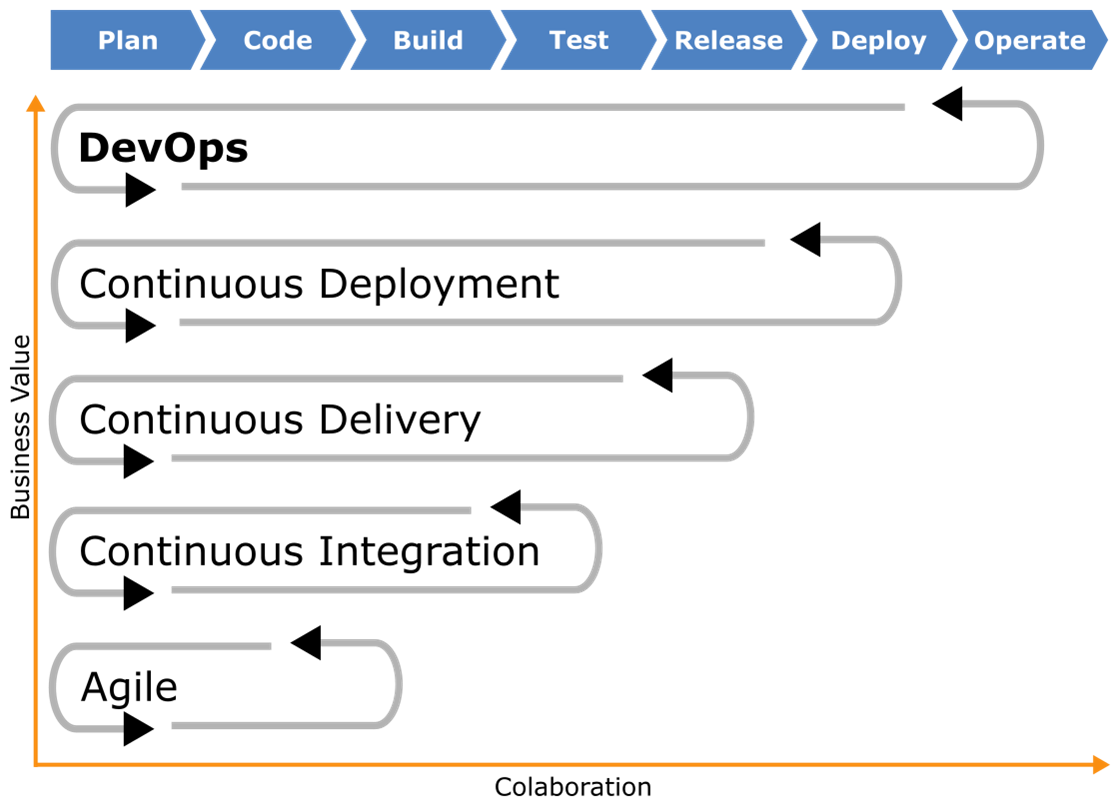
\includegraphics[scale = 0.2]{img/devops0.png} & 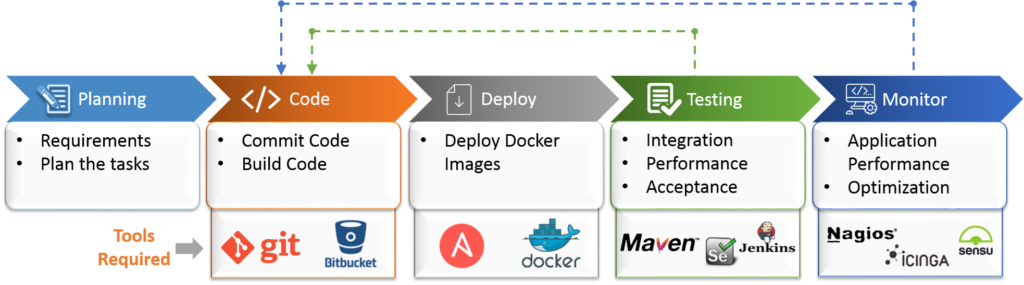
\includegraphics[scale = 0.35]{img/devops1.png}
\end{tabular}


%%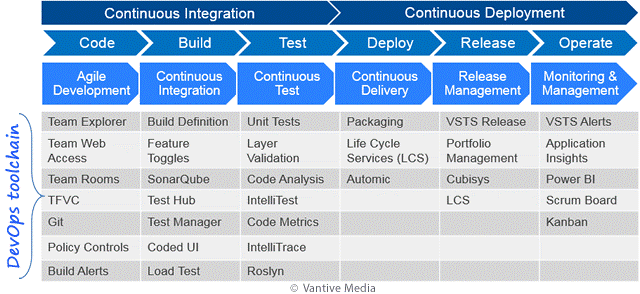
\includegraphics[scale = 0.6]{img/bls18/devops.png}

%-----------------------------------------------------
\subsection{Bottom-up or Top-Down?}
\labelssec{bottomtop}
%-----------------------------------------------------

\begin{tabular}{ | c | c | c | }
     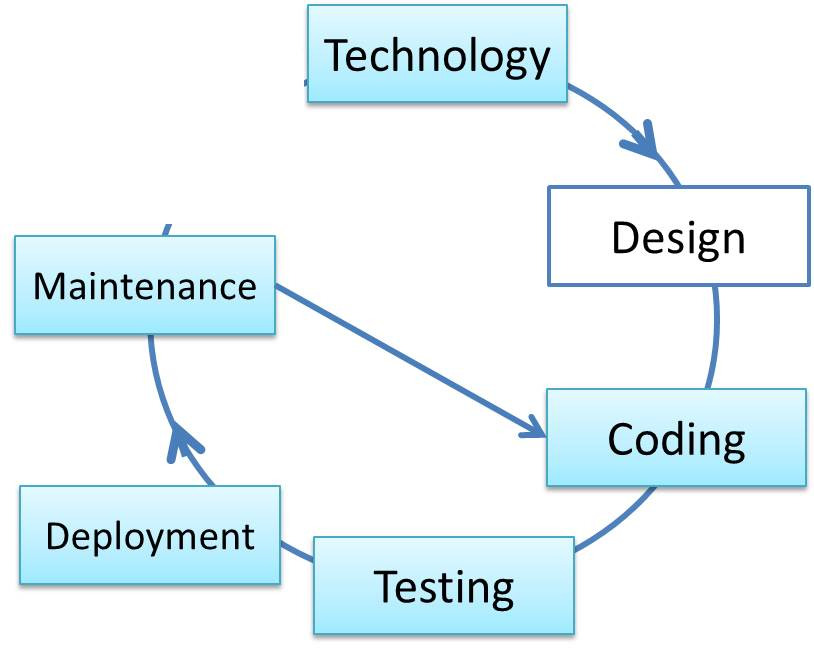
\includegraphics[scale = 0.35]{img/introDesign1.jpg} & 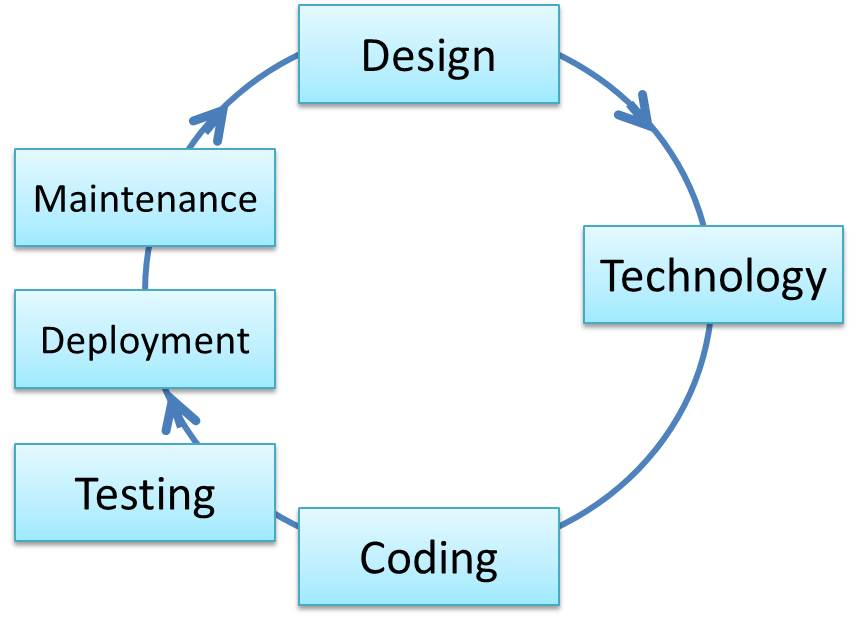
\includegraphics[scale = 0.35]{img/introDesign2.jpg} & 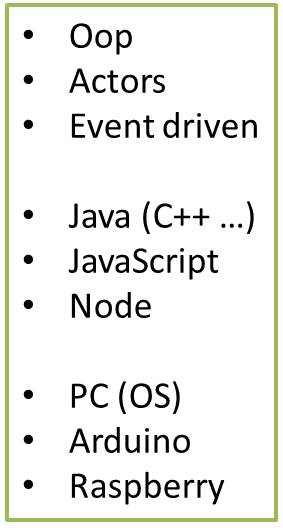
\includegraphics[scale = 0.35]{img/introDesignTecno.jpg}
\end{tabular}


\newpage 
%===========================================================================
\section{Technology-based design}
\labelsec{blstechnobased}
%===========================================================================

The button is a source that emits a wave that can be sampled. 
\medskip 

\begin{tabular}{ c }
     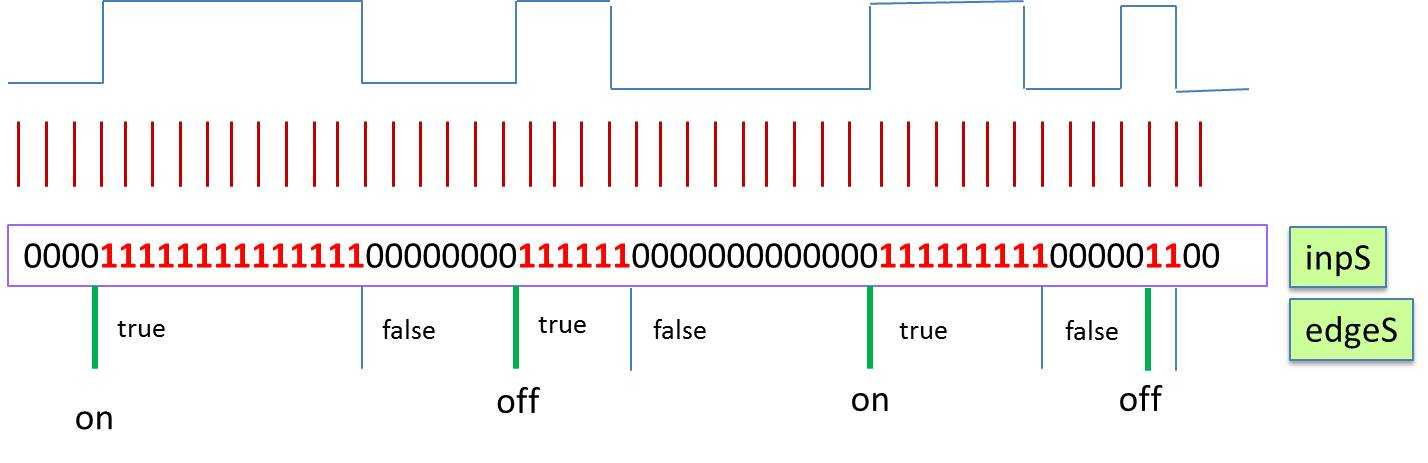
\includegraphics[scale = 0.45]{img/buttonLedWave.jpg}
\end{tabular}

 

At this level, the problem requires that the following elaborations on the basic input 
\begin{itemize}
\item the detection of the edges in the input sequence
\item the detection of edges of type "low to high"  
\end{itemize}

%-----------------------------------------------------
\subsection{Function-based software}
\labelssec{fun}
%-----------------------------------------------------
The responsibility of these functions can be given to two new different entities: an entity \textit{EdgeDetector} and an entity \textit{Controller} that realizes the "business logic" of the system. 
%%In particular, the \textit{Controller}) receives in input the sequence \texttt{edgeS} and performs a \textit{switch} of the led for each \texttt{true} value found in the input sequence.

\begin{tabular}{ c }
     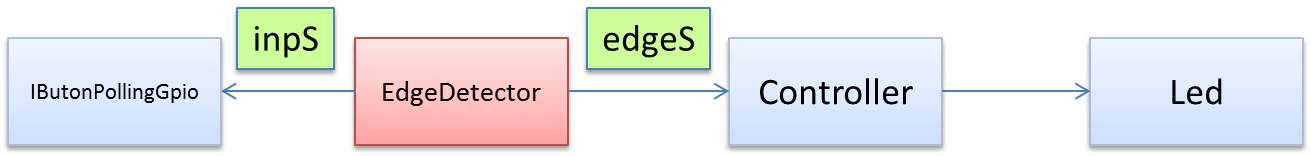
\includegraphics[scale = 0.55]{img/buttonLedLogic0.jpg}
\end{tabular}


The code can be structured in imperative style, by using \code{functions} as a first kind of software component:

\begin{tabular}{|c|c|}
\hline 
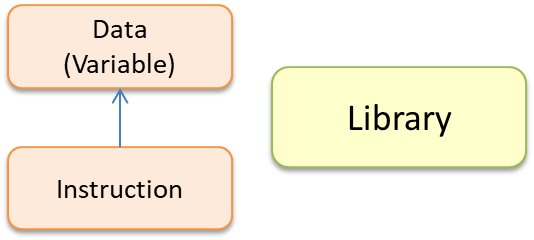
\includegraphics[scale = 0.4]{img/c0.png} &  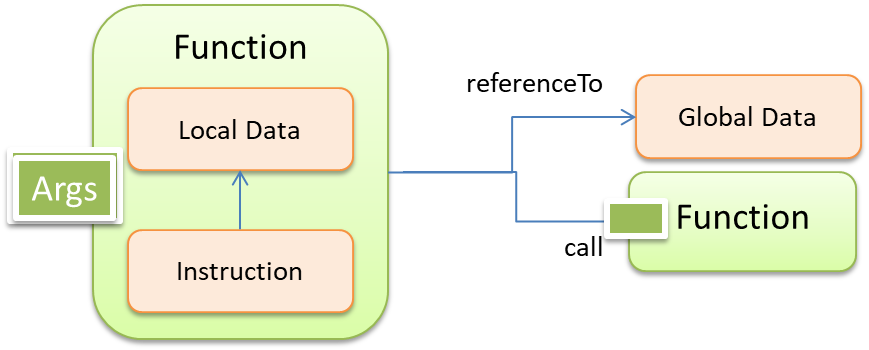
\includegraphics[scale = 0.4]{img/c1.png}\\
\hline 
\end{tabular}

If an (application) function is called each time a new input becomes available, the system is 'reactive' or \code{event-driven}.



%-----------------------------------------------------
\subsection{Object-based software}
\labelssec{obj}
%-----------------------------------------------------
As an alternative of the function-based code of \xss{fun}, both the \textit{EdgeDetector} and the \textit{Controller} can be modelled as finite state machines (\texttt{FSM}) working as \textit{transducers}. 
They can be viewed as \textit{objects} interacting via procedure-calls.
%% or \textit{active entities} (e.g. processes, actors, agents, etc) interacting via message-passing.


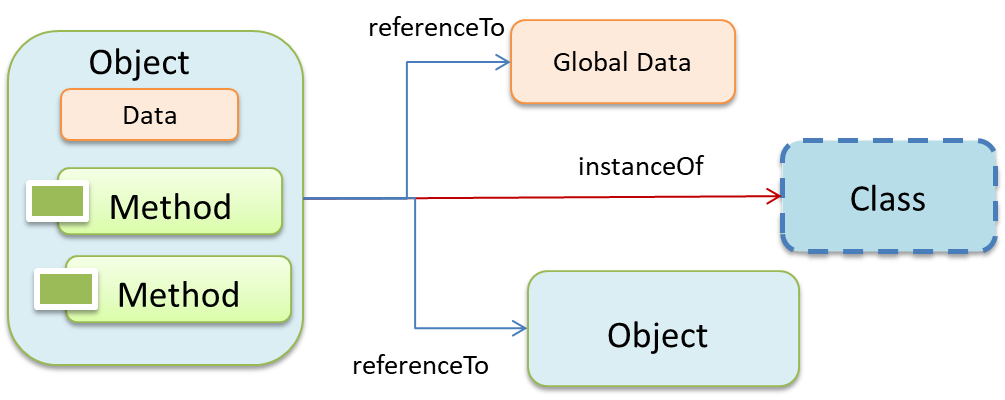
\includegraphics[scale = 0.4]{img/c2.png}

In any object-oriented model, all the computation usually takes place within a single thread. In our case the main thread could be the thread related to the component that performs the polling of the wave, i.e. the  \texttt{EdgeDetector}.  In this case, the \textit{Controller} is called by the \textit{EdgeDetector} that, must explicitly know the \textit{Controller} in order to call it. 

%-----------------------------------------------------
\subsection{Observable and Observers}
\labelssec{Observers}
%-----------------------------------------------------

A more flexible architecture an be obtained (without changing the run-time interaction pattern) by conceiving the \textit{Controller} as an \textit{observer} that can be registered to the \textit{EdgeDetector} information source. 

\medskip 
\begin{tabular}{|c|}
\hline 
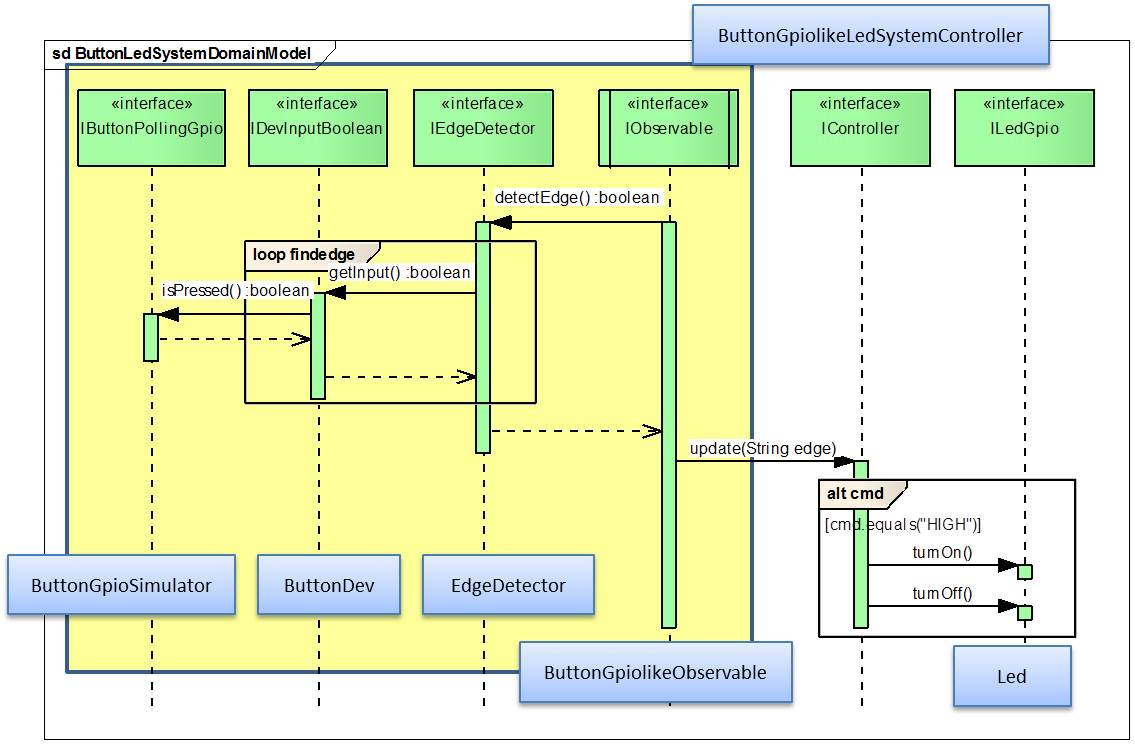
\includegraphics[scale = 0.55]{img/buttonLedInteraction1.jpg}\\
\hline 
\end{tabular}



\medskip 
\footnotesize
\framebox[14cm]{ %
\begin{minipage}{135mm}
However, staring from the idea that a Button is an 'edge detector' device is a too low-level approach for modern software applications. An effort has to be made to introduce a more appropriate \code{model} of the \texttt{Button} entity in terms of structure, interaction and behavior.
\end{minipage}}
\normalsize
\medskip 


%-----------------------------------------------------
\subsection{Models }
\labelssec{models}
%-----------------------------------------------------

\medskip 
\begin{tabular}{|c|c|}
\hline 
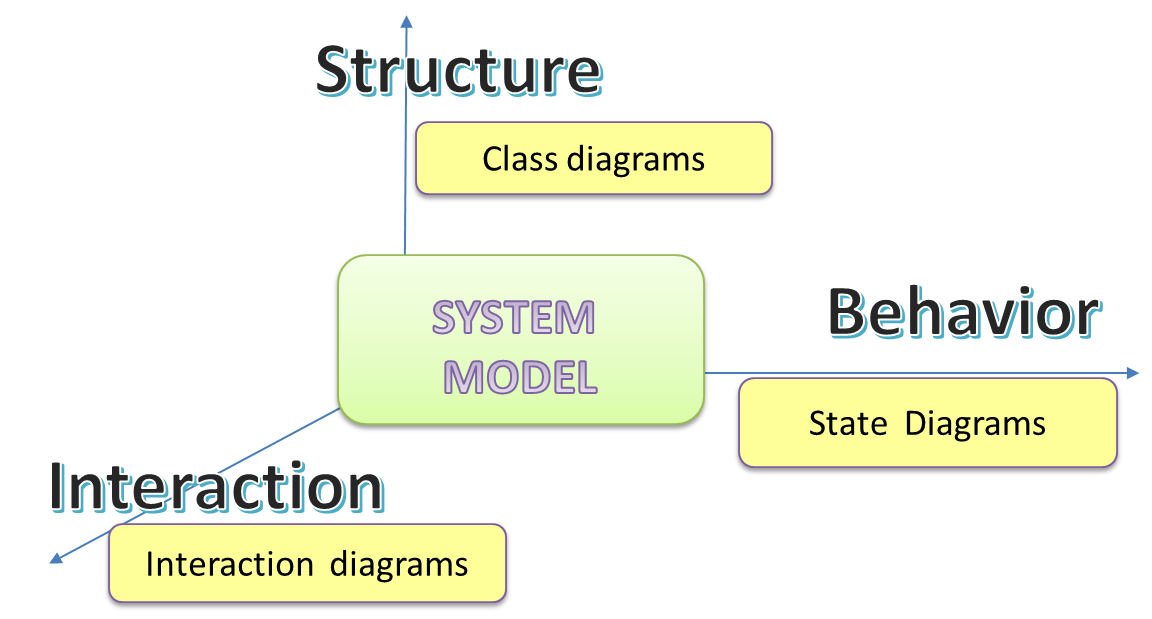
\includegraphics[scale = 0.3]{img/sib.png} &  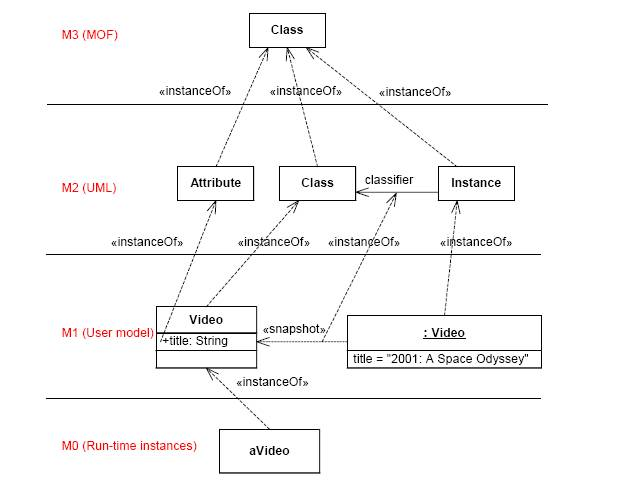
\includegraphics[scale = 0.4]{img/unl2MetaHierExample.jpg}\\
\hline 
\end{tabular}
\medskip 


%-----------------------------------------------------
\subsection{Modelling a Button }
\labelssec{buttonmodel}
%-----------------------------------------------------

\footnotesize
From the \code{structural} point of view, a button is intended by a customer as an \textit{\fname{atomic}} entity whose \code{behavior} can be modelled as a \textit{\fname{finite state machine}} (\code{FMS}) composed of two states ( '\texttt{pressed}' and '\texttt{unpressed}'). The state transition is performed by some agent \textit{external} to the system (an user, a program, a device, etc.). From the \code{interaction} point of view, the button can expose its internal state in different ways:

\begin{itemize}
\item by providing a \fname{property} operation (e.g. \texttt{boolean isPressed()}) that returns \texttt{true} when the button is in the \texttt{pressed} state. In this way the interaction is based on  "\code{polling}";
\item by providing a \fname{synchronizing} operation (e.g. \texttt{void waitPressed()}) that blocks a caller until the button transits in the  \textbf{pressed} state. In this way the interaction is based conventional  "\code{procedure-call}";
\item by working as an \fname{observable} according to the \textit{Observer} design pattern. In this way the interaction is based on "\code{inversion of control}" and involves observers (also called "\textit{listeners}") that must be explicitly referenced (via a "\textit{register}" operation) by the button.
\item by emitting \fname{events} handled by an event-based support. In this way the interaction is based on "inversion of control" that involves observers (usually known as "\textit{callbacks}") referenced by the support and not by the button itself.
\item by sending \fname{messages} handled by a message-based support. In this way the interaction is based on message passing and can follow different "patterns" (in our internal terminology we distinguish between \textit{dispatch}, \textit{invitation}, \textit{request-response}, etc.)
\end{itemize}


All these "models" could be appropriate in some software application. Thus, a very useful exercise is to define in a formal way each of these models by adopting (at the moment) a test-driven approach.

\normalsize

\newpage 
%===========================================================================
\section{An object-based design}
\labelsec{blsoo}
%===========================================================================

Working in the conceptual space of 'classical' object oriented software development, the logic architecture of the \code{BLS} can be summarized by the following \uml{} interaction diagram:

\medskip 
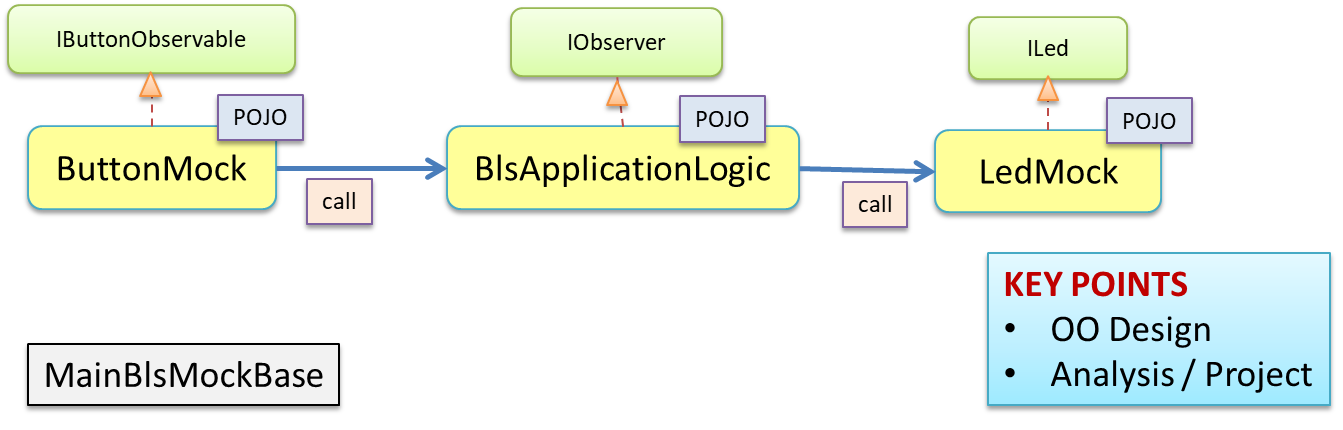
\includegraphics[scale = 0.3]{img/bls18/bls18Obj0.png}
\medskip 
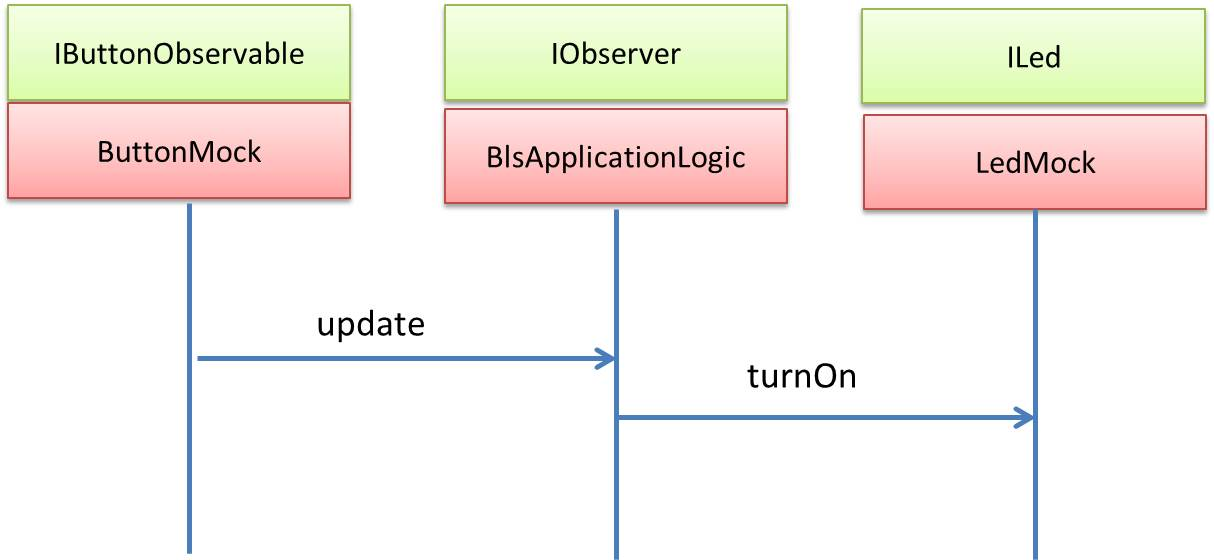
\includegraphics[scale = 0.3]{img/blsSeqUML.jpg}
\medskip 
 


The computation starts from the observable device (\textit{Button}), that calls a method of the object devoted to implement the application logic (that works as the \texttt{Observer}).
An example is given in the project \code{it.unibo.bls.oo} that is based on the \java{} lanaguage. The working directory of the project is structured as follows:

\footnotesize
\begin{itemize}
\item The package \code{it.unibo.bls.interfaces} includes the definition of the object interfaces.
\item The package \code{it.unibo.bls.devices} includes the implementation of the object interfaces related to the devices (\texttt{Button} and \texttt{Led}). For each device, two different implementations are given: a \texttt{Mock} device and a 'virtual' object implemented with a \texttt{GUI}. 
\item The package \code{it.unibo.bls.applLogic} includes the definition of the object that implements the application logic.
\item The package \code{it.unibo.bls.appl} includes the \texttt{Main} programs.
\item The \code{test} directory includes examples of test units.
\end{itemize}
\normalsize

 
A software system working with the \texttt{Mock} devices should include a \code{configuration phase} to create the system components (objects) and properly connect them, according to the system architecture design:

 %%C:\Didattica2018Work\iss2018Lab\it.unibo.bls18\src\it\unibo\bls\appl\MainBlsMockBase.java
 
\lstinputlisting[language=Java, caption={ \texttt{MainBlsMockBase.java}: configuration }, firstline=9, lastline=24 ]{../../src/it/unibo/bls/devices/mock/MainBlsMockBase.java} 
 
The system defines also some working activity, to cause the change of the state in the \texttt{ButtonMock}:

\lstinputlisting[language=Java, caption={ \texttt{MainBlsMockBase.java}: simulated action }, firstline=25, lastline=31 ]{../../src/it/unibo/bls/devices/mock/MainBlsMockBase.java} 

Since every system is a \textbf{composed} (i.e. it is a \code{non-atomic}) entity, it provides also \textbf{selector-methods} to get its components:

\lstinputlisting[language=Java, caption={ \texttt{MainBlsMockBase.java}: selectors }, firstline=32, lastline=37 ]{../../src/it/unibo/bls/devices/mock/MainBlsMockBase.java} 

The selectors can be useful during the testing, to access the state of the single devices.

Finally, there is the \code{main} method:
\lstinputlisting[language=Java, caption={ \texttt{MainBlsMockBase.java}: the main method}, firstline=38, lastline=42 ]{../../src/it/unibo/bls/devices/mock/MainBlsMockBase.java} 

\newpage 
%=================================================================
\section{From BLS Mock devices to physical devices}
\labelsec{blsphysical}
%=================================================================
The logical architecture previously introduced does not change if we replace the \texttt{Mock} devices with concrete devices: For example, in the case of virtual devices implemented with a \texttt{GUI}:


\medskip 
\begin{tabular}{|c|c|}
\hline 
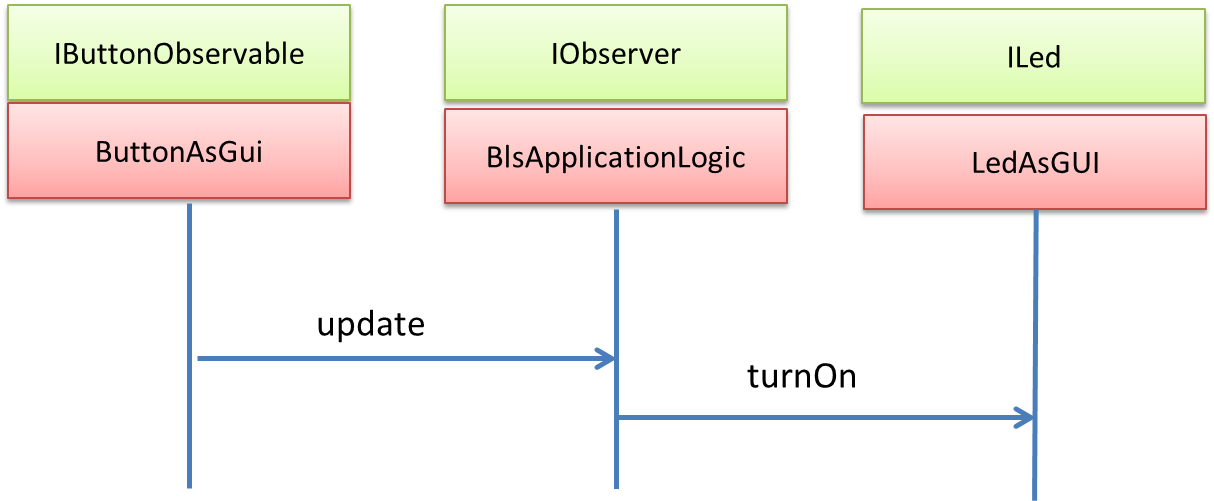
\includegraphics[scale = 0.3]{img/blsGuiUM.png} &  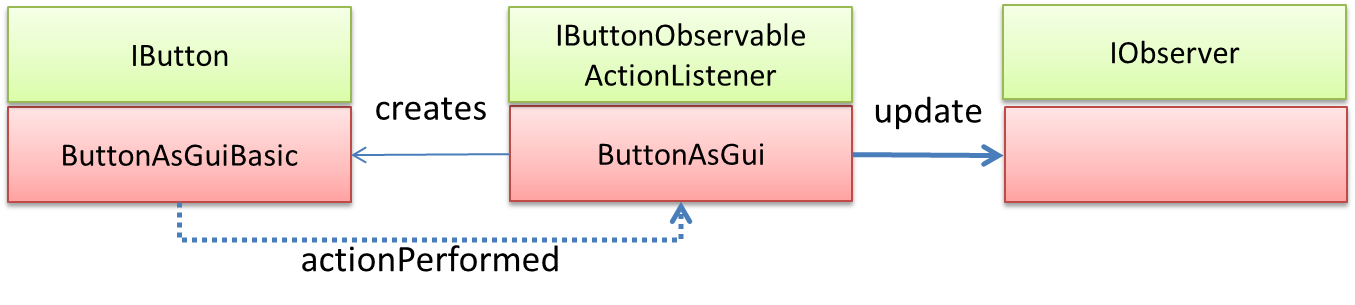
\includegraphics[scale = 0.3]{img/buttonGuiUM.png}\\
\hline 
\end{tabular}
\medskip 

The class \code{ButtonAsGuiBasic} implements a \texttt{GUI}-based Button by extending the class \code{java.awt.Button}. The class \code{ButtonAsGui} implements the concept of \texttt{Button} as \texttt{Observable} entity. 

Note that \code{ButtonAsGui} re-uses the class \code{ButtonAsGuiBasic} but without exploiting inheritance. Rather, it creates an instance of  \code{ButtonAsGuiBasic} and works as its listener.  This behaviour is caused by the fact that \java{} does not support multiple inheritance for classes and \code{ButtonAsGui} already extends the class \code{java.util.Observable}.

In a more general perspective, we could build this part of our software system by exploiting the \code{Dependency Injection} pattern.
 
\subsubsection{Dependency injection and Inversion of Control}.\\
In software engineering, an \code{injection} is the passing of a dependency to a dependent object (a client) that would use it as a service. In the \code{dependency injection} pattern, passing the service to the client, rather than allowing a client to build or find the service, is the fundamental requirement.

\noindent
\footnotesize
\framebox[14cm]{ %
\begin{minipage}{135mm}
Dependency injection is one form of the broader technique of \code{Inversion of Control}. The client delegates the responsibility of providing its dependencies to external code (the \code{injector}). The client is not allowed to call the injector code.  
\end{minipage}}
\normalsize
\medskip 


\medskip 
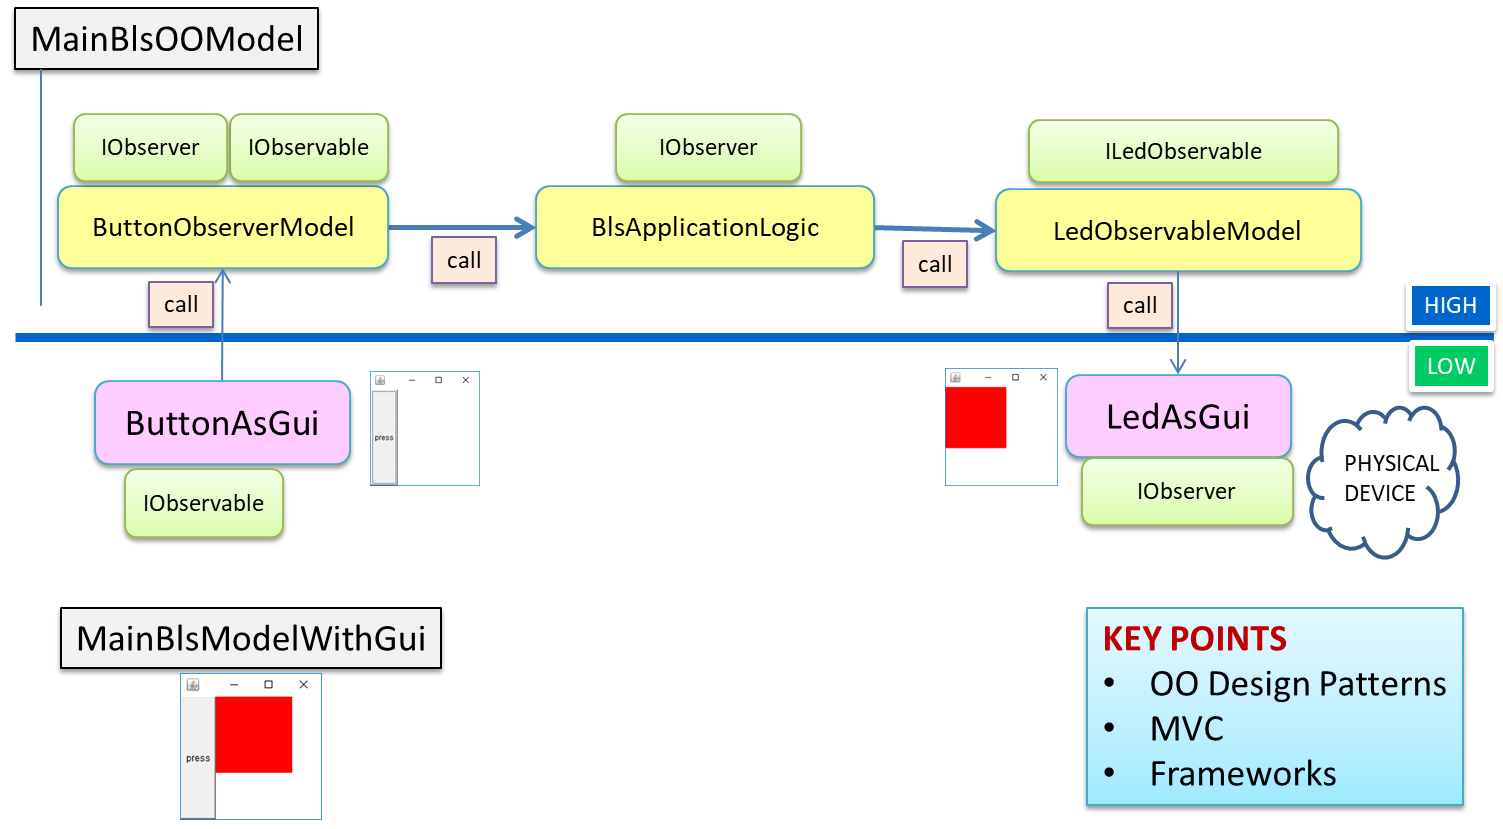
\includegraphics[scale = 0.5]{img/bls18/bls18Obj1.png}


%% MainBlsModelWithGui

%-----------------------------------------------------------------------
\subsection{MVC}
\labelssec{mvc}
%-----------------------------------------------------------------------
\medskip 
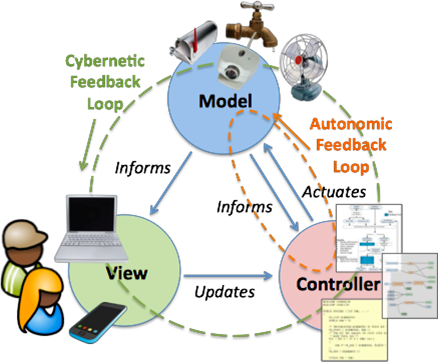
\includegraphics[scale = 0.5]{img/mvc.png}


%-----------------------------------------------------------------------
\subsection{Devices on Arduino}
\labelssec{devonarduino}
%-----------------------------------------------------------------------

\medskip 
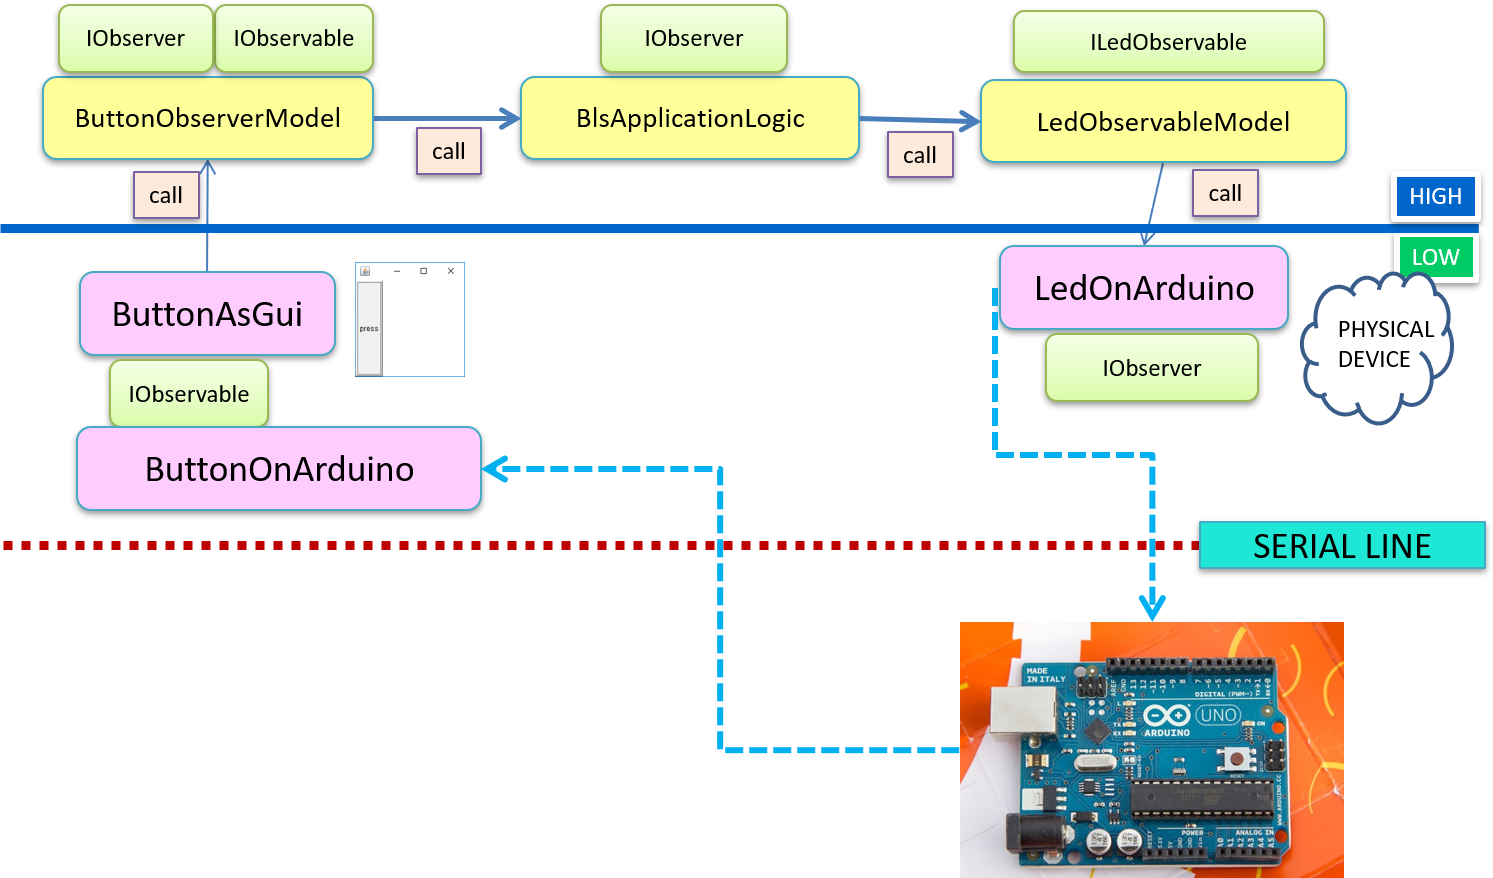
\includegraphics[scale = 0.5]{img/bls18/bls18Obj2Arduino.png}

%% MainBlsModelWithArduino 

%-----------------------------------------------------------------------
\subsection{Devices on Raspberry}
\labelssec{devonarduino}
%-----------------------------------------------------------------------

\medskip 
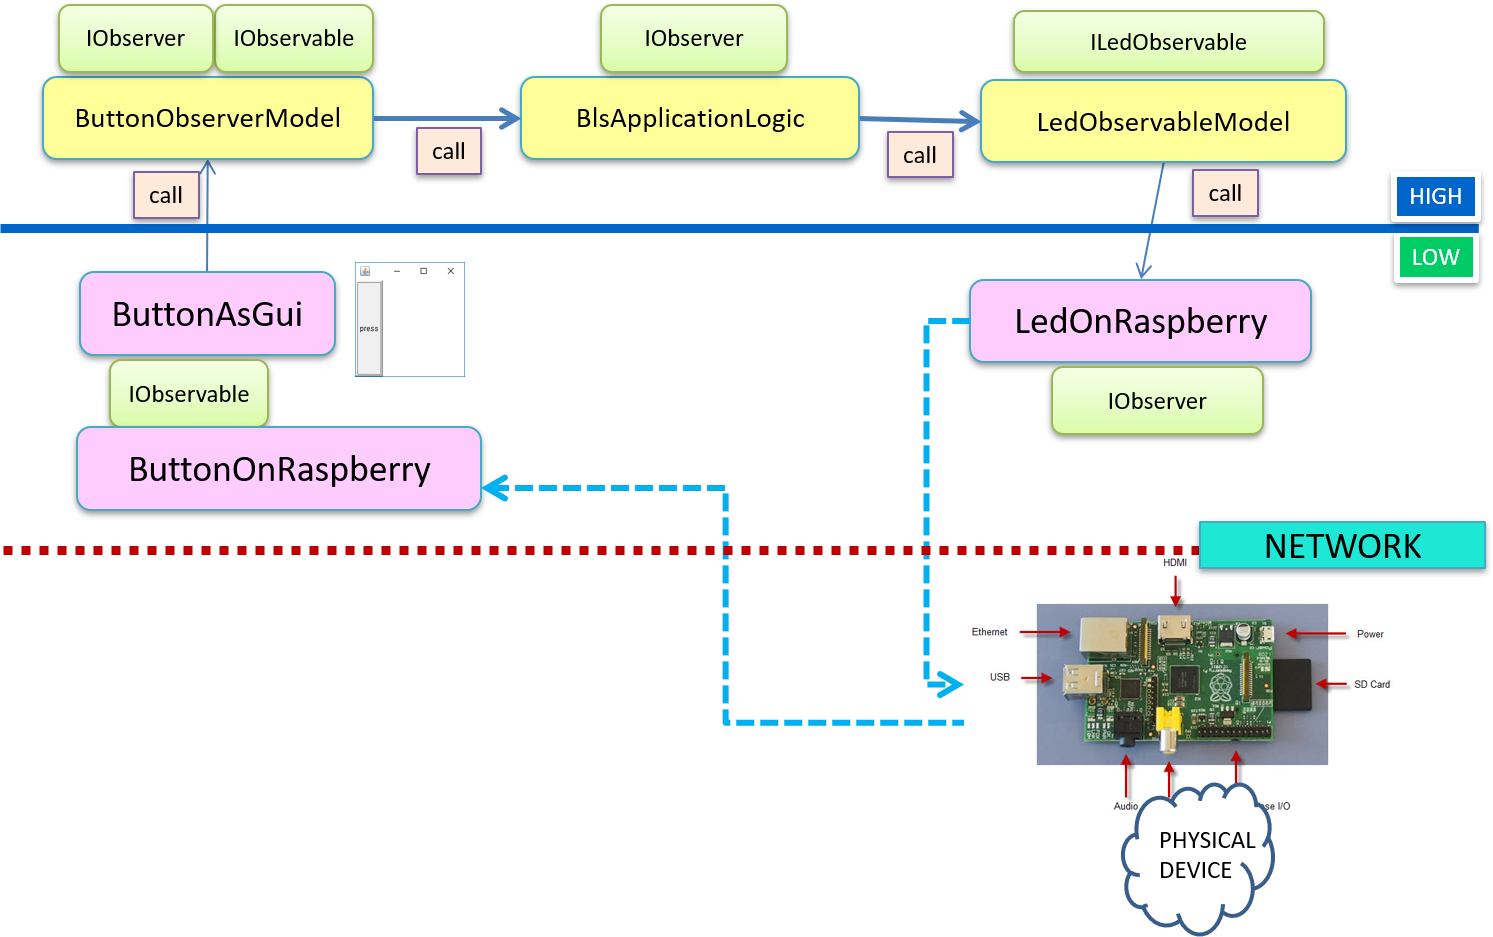
\includegraphics[scale = 0.5]{img/bls18/bls18Obj2Rasp.png}

%% MainBlsModelWithArduino 

%-----------------------------------------------------------------------
\subsection{IOT}
\labelssec{iot}
%-----------------------------------------------------------------------
\medskip 
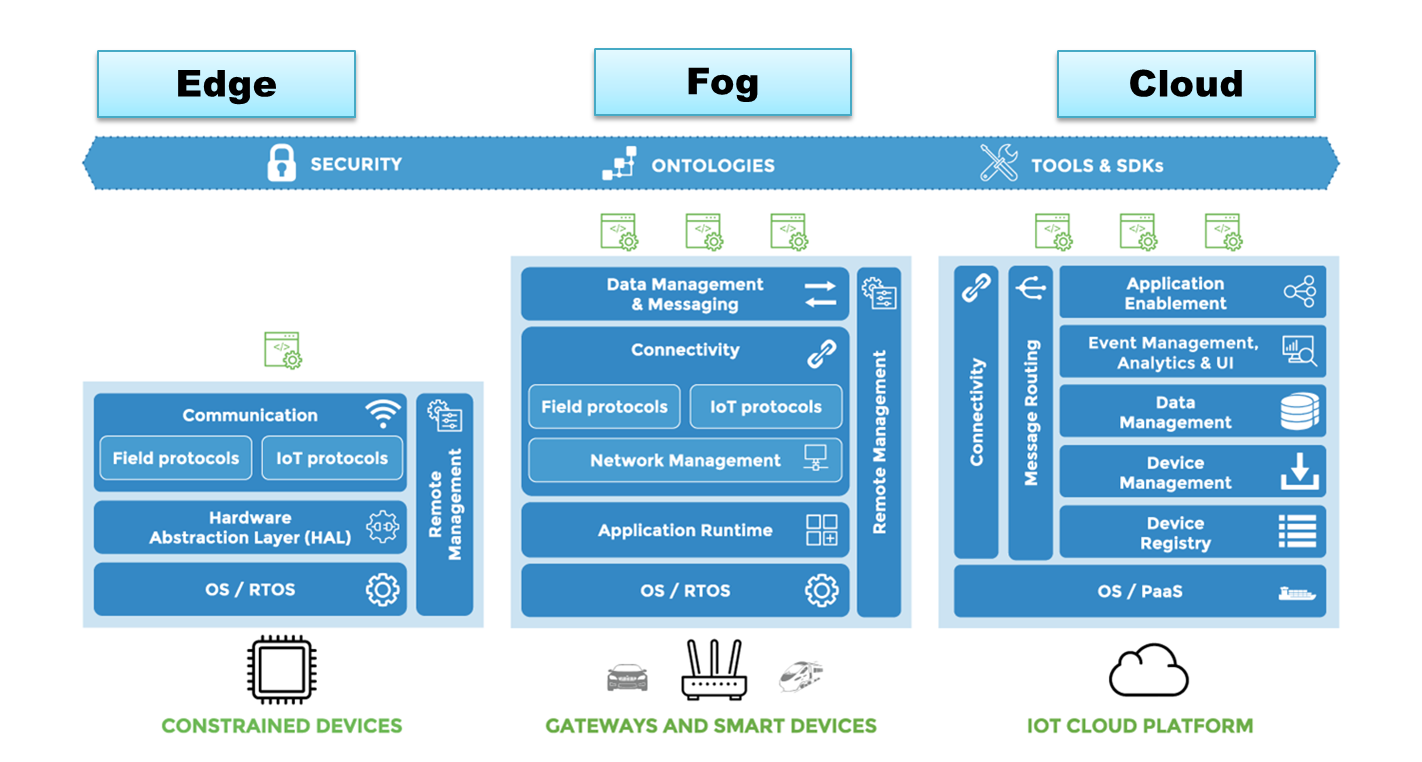
\includegraphics[scale = 0.5]{img/iot3TecnoStack.png}

%-----------------------------------------------------------------------
%% \subsection{From a BLS local system to a BLS distributed}
%%\labelssec{blsdistributed}
%-----------------------------------------------------------------------

%\includegraphics[scale = 0.5]{img/bls18/bls18/obj1.png}

\newpage
%===========================================================================
\section{Evolving the BLS into a distributed system}
\labelsec{blsdistributed}
%===========================================================================

 \medskip 
\begin{tabular}{|c|c|}
\hline 
\includegraphics[scale = 0.6]{img/obj1.png} &  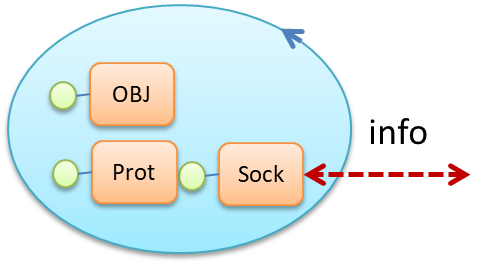
\includegraphics[scale = 0.7]{img/obj2.png}\\
\hline 
\end{tabular}
\medskip 
 

%-----------------------------------------------------------------------
\subsection{Led as a remote devices: the proxy pattern }
\labelssec{ledremote}
%-----------------------------------------------------------------------

\medskip 
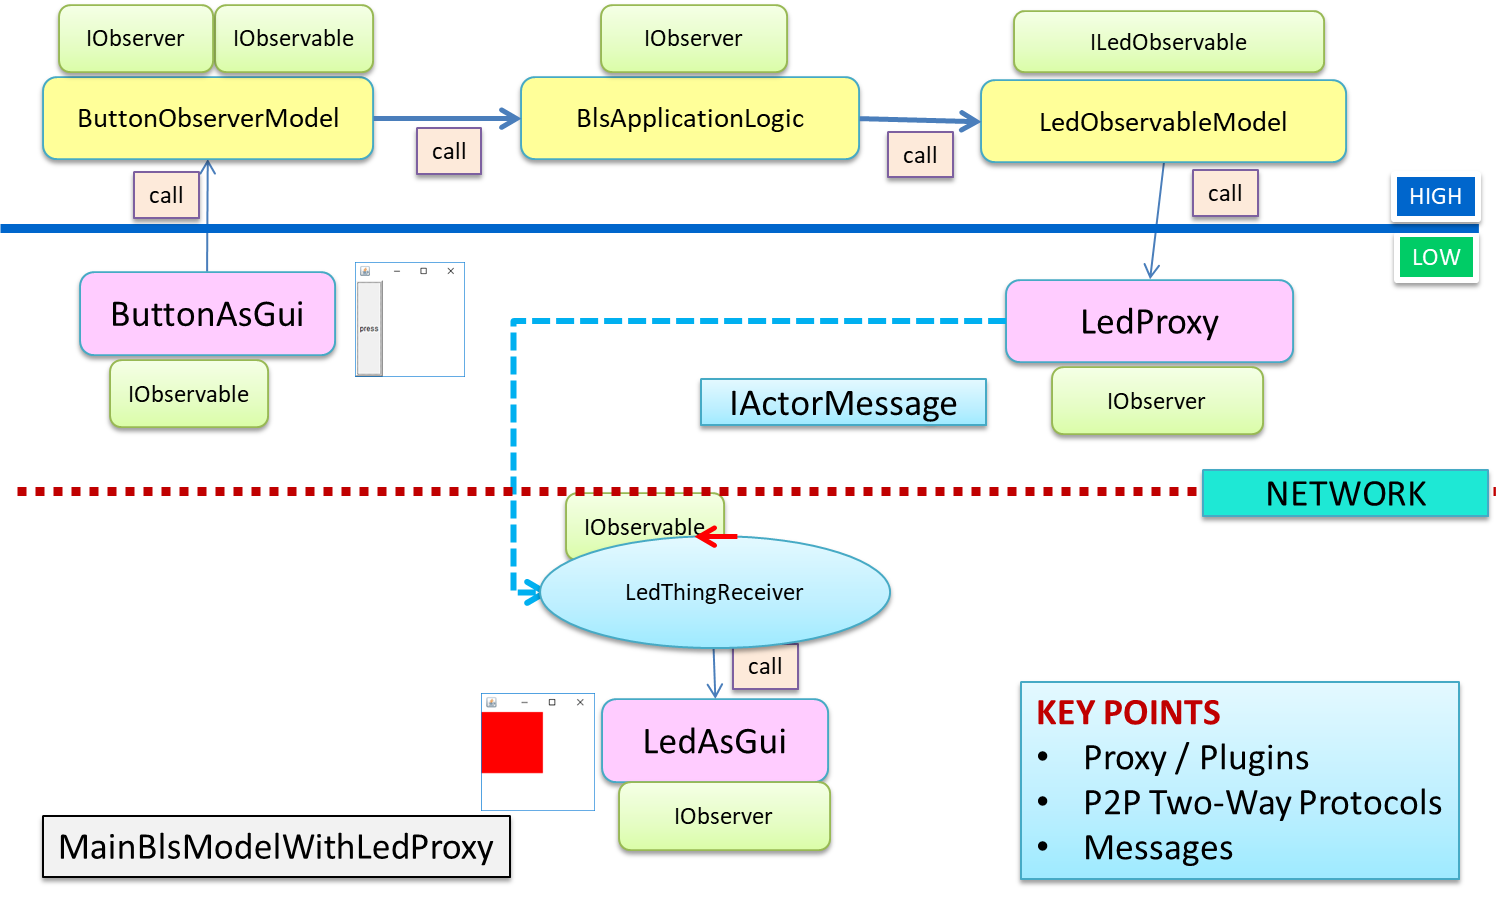
\includegraphics[scale = 0.5]{img/bls18/bls18ObjLedRemote.png}

%% MainBlsModelWithLedProxy 

%-----------------------------------------------------------------------
\subsection{Led as a remote device. the publish-subscribe pattern }
\labelssec{mqtt}
%-----------------------------------------------------------------------

\medskip 
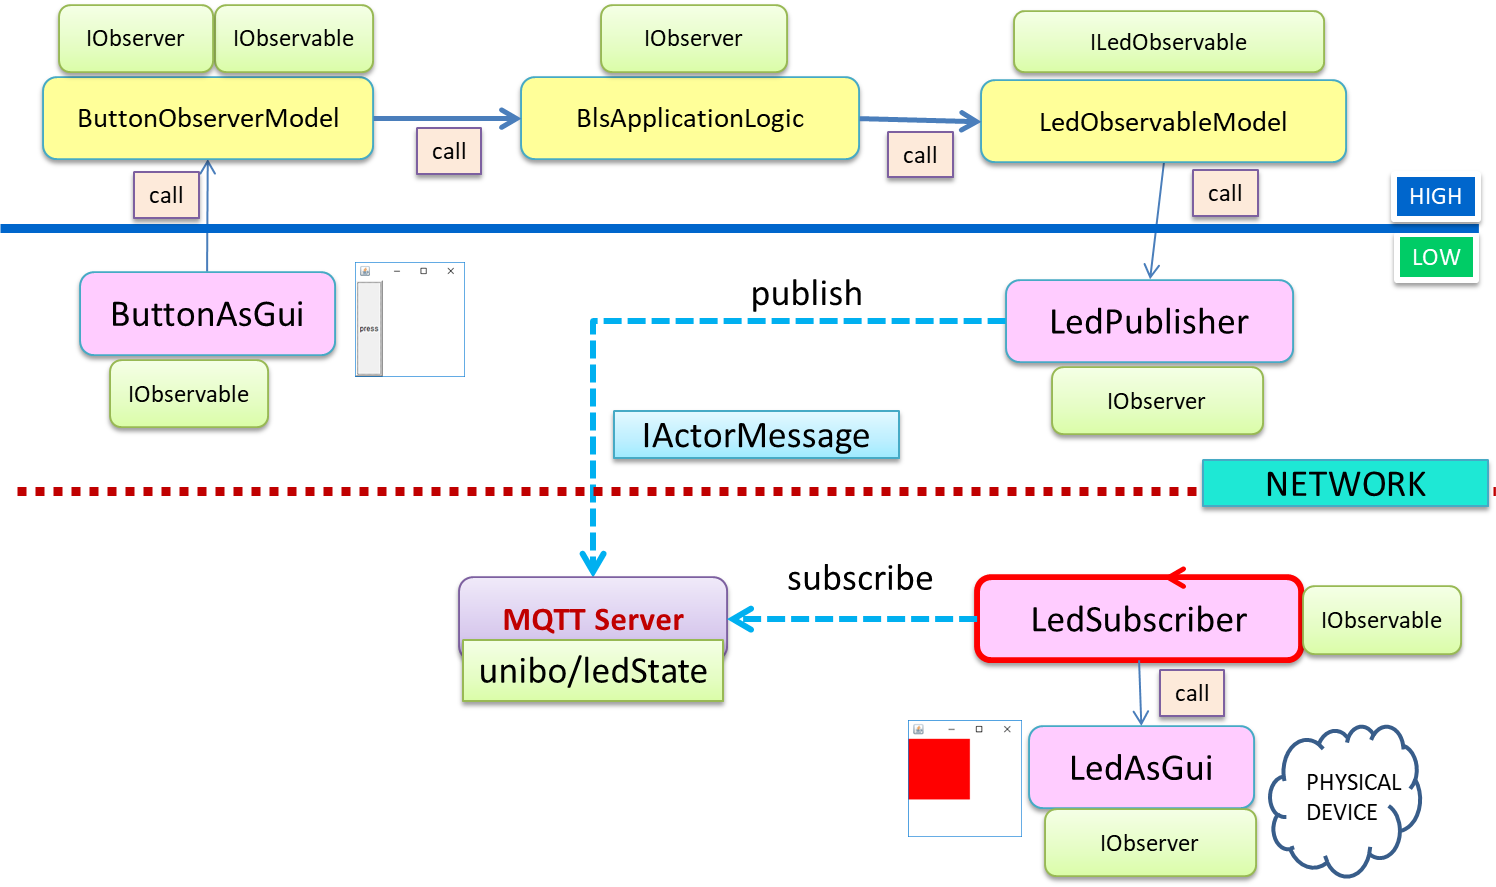
\includegraphics[scale = 0.5]{img/bls18/bls18ObjLedMqtt.png}

%% MainBlsModelMqtt 

\newpage 
%===========================================================================
\section{CoAP}
\labelsec{coap}
%===========================================================================
 
\medskip 
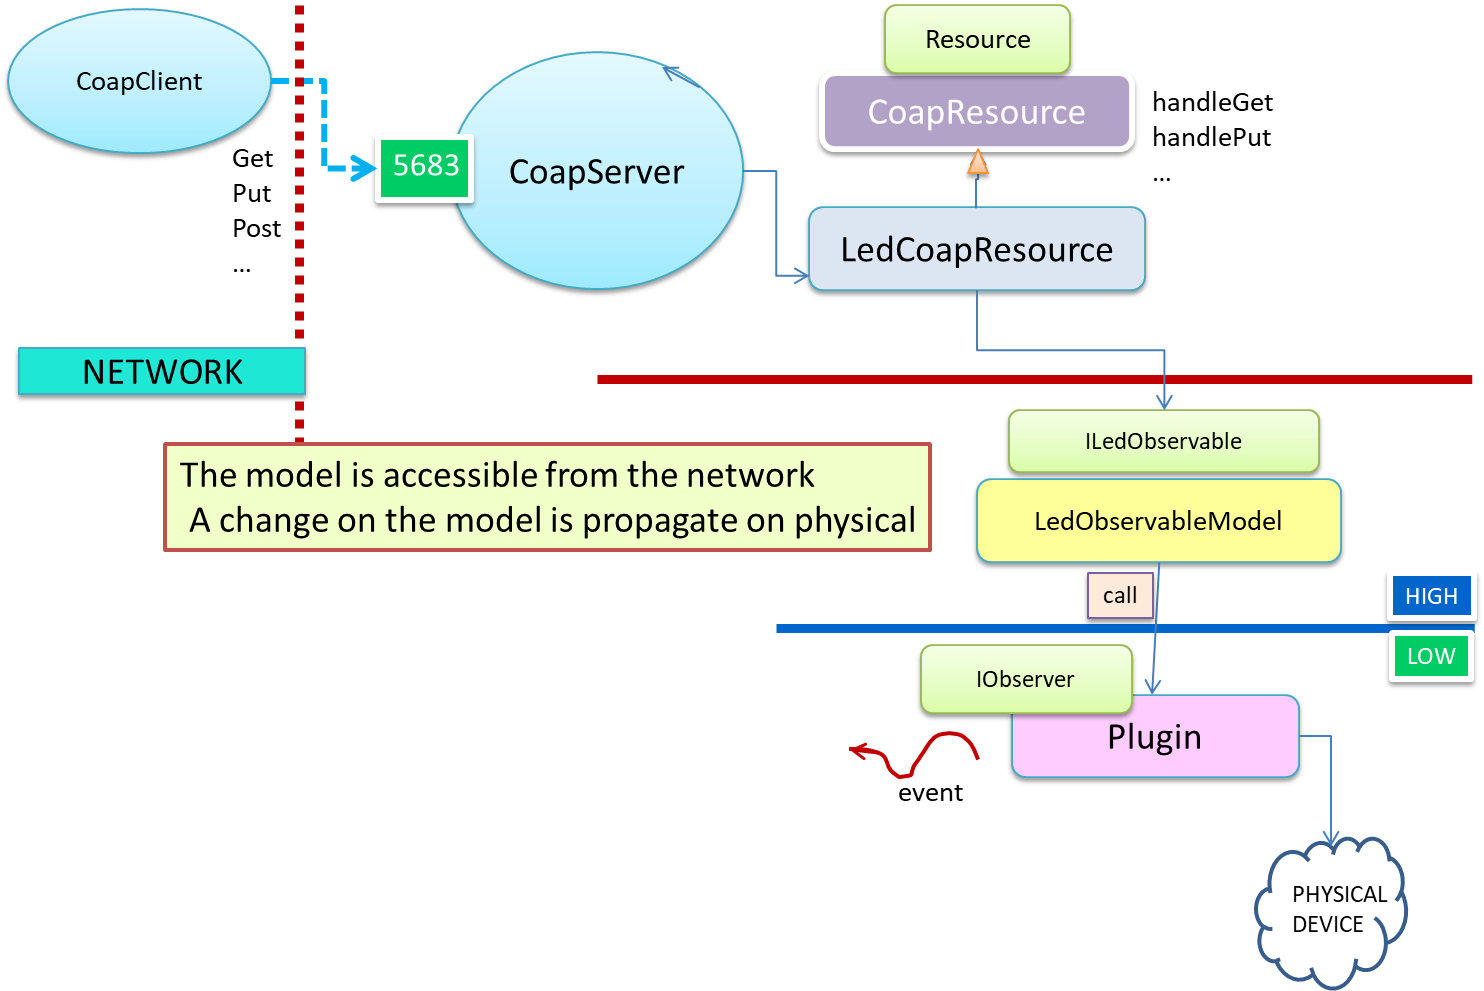
\includegraphics[scale = 0.5]{img/bls18/bls18Coap0.png}

%% MainCoapBasicLed 


%-----------------------------------------------------------------------
\subsection{Led as a (CoAP) thing }
\labelssec{coapled}
%-----------------------------------------------------------------------

\medskip 
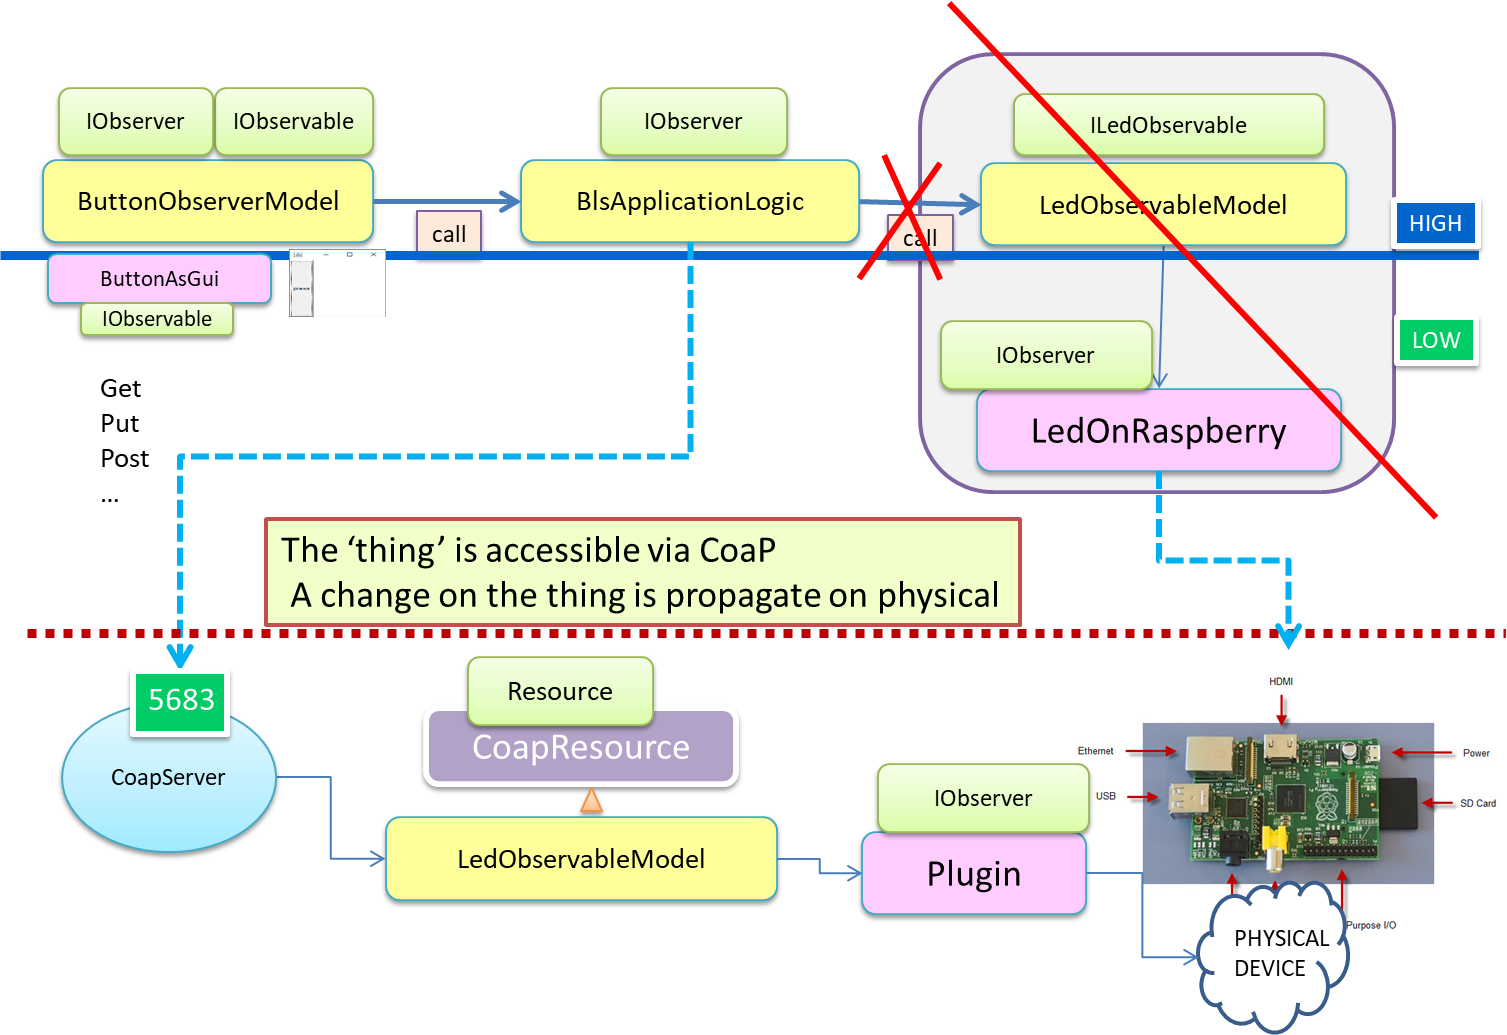
\includegraphics[scale = 0.5]{img/bls18/bls18CoapBL.png}

%% MainCoapControlToLedRest

%-----------------------------------------------------------------------
\subsection{Hexagonal srchitecture}
\labelssec{hex}
%-----------------------------------------------------------------------
\medskip 
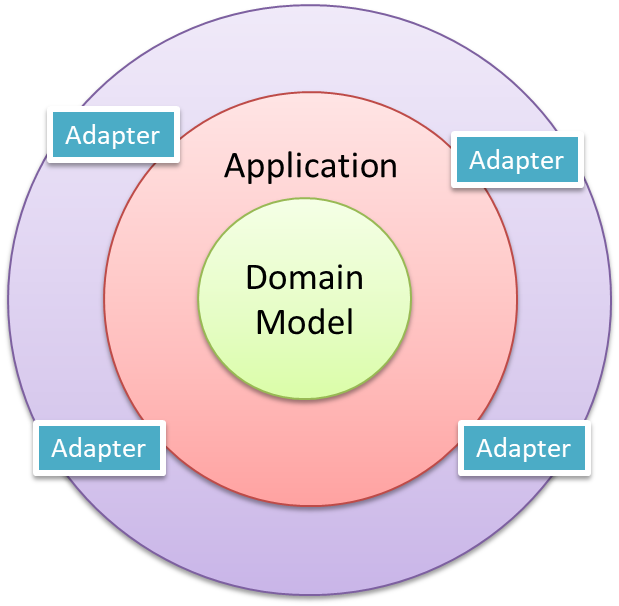
\includegraphics[scale = 0.5]{img/hex1.png}

\medskip 
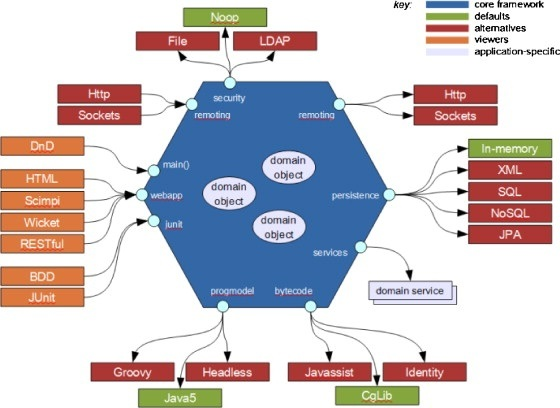
\includegraphics[scale = 0.5]{img/hex3.png}



%-----------------------------------------------------------------------
\subsection{BLS front end }
\labelssec{coapfrontend}
%-----------------------------------------------------------------------

\medskip 
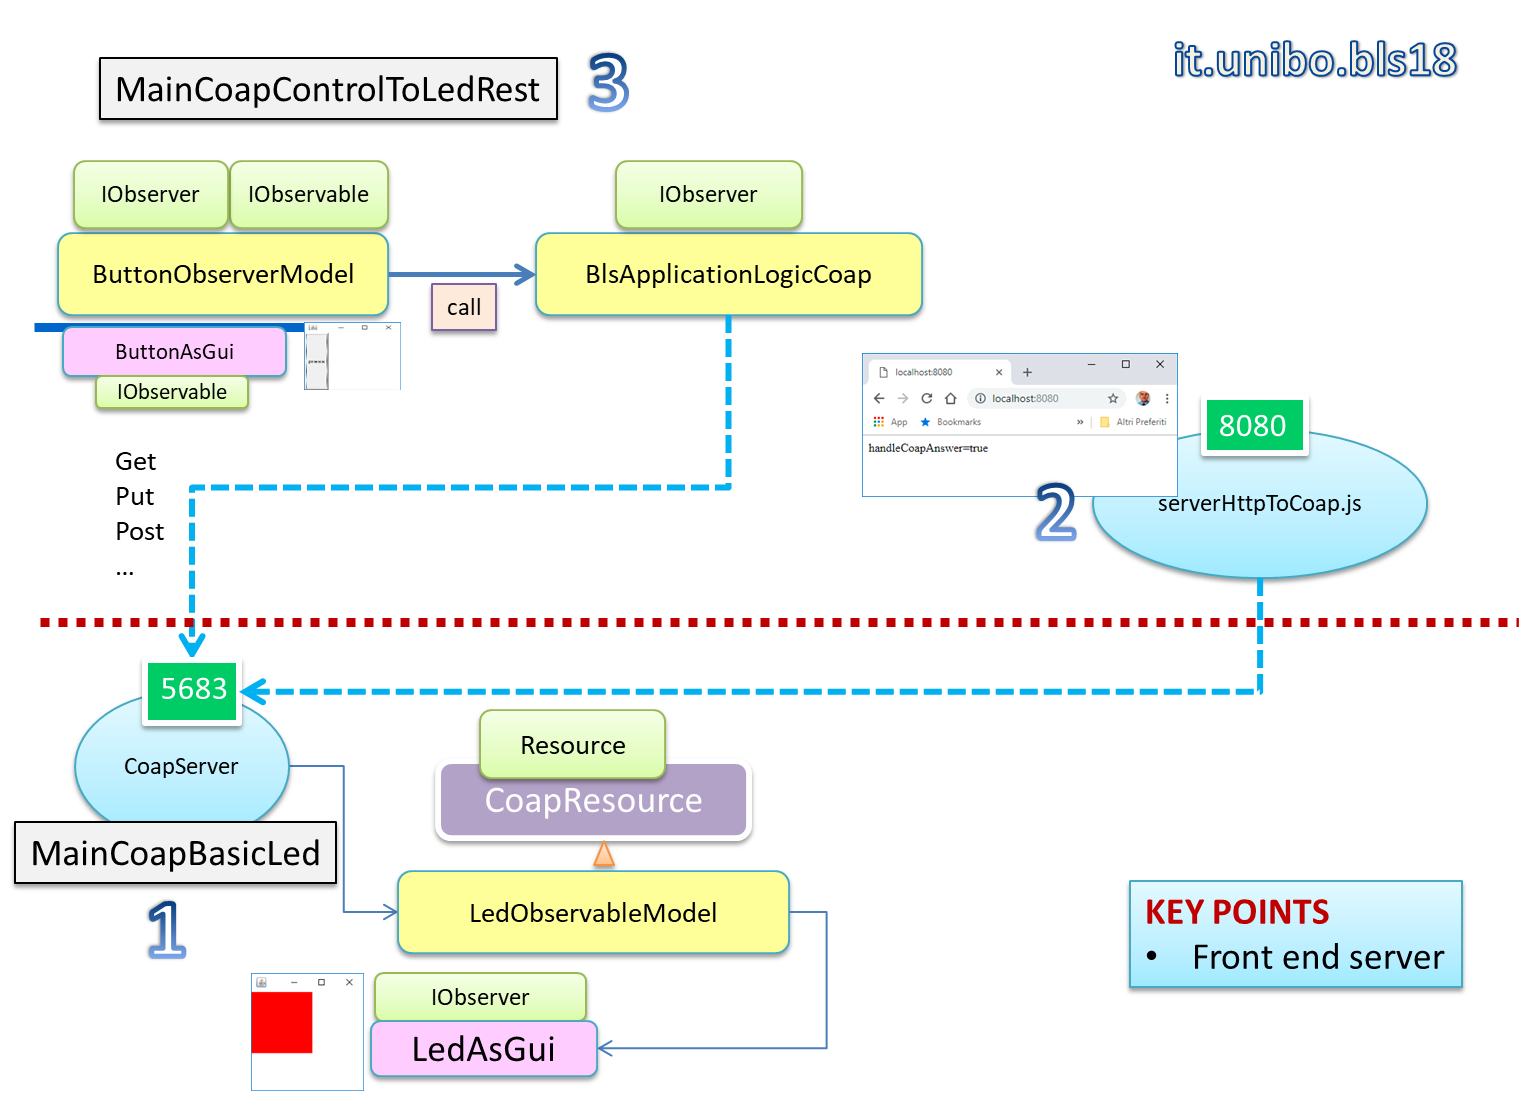
\includegraphics[scale = 0.5]{img/bls18/bls18CoapFrontEnd.png}

 

\end{document}